\documentclass[11pt,a4paper]{article}
\usepackage[utf8]{inputenc}
\usepackage[T1]{fontenc}
\usepackage{amsmath,amssymb,amsfonts}
\usepackage{geometry}
\geometry{left=1.25cm,right=1.25cm,top=1.25cm,bottom=3.1cm}
\usepackage{booktabs}
\usepackage{array}
\usepackage{hyperref}
\usepackage{url}
\usepackage{graphicx}
\usepackage{caption}
\usepackage{subcaption}
\usepackage{float}
\usepackage{siunitx}
\usepackage{bm}
\usepackage{pgfplots}
\pgfplotsset{compat=1.18}
\usepackage{xcolor}
\usepackage{titlesec}
\usepackage{fancyhdr}
\usepackage{microtype}
\usepackage{multicol}
\usepackage{fontspec}
\setmainfont{Calibri}
\setsansfont{Calibri}
\setsansfont{Segoe UI}[
BoldFont = Segoe UI Bold,
Ligatures = TeX
]

\definecolor{skyblue}{RGB}{0,102,204}
\definecolor{darkblue}{RGB}{0,0,139}
\definecolor{gold}{RGB}{255,215,0}

\newcommand{\eps}{\varepsilon}
\newcommand{\kappac}{\kappa_c}
\newcommand{\Keff}{K_{\mathrm{eff}}}
\newcommand{\betaf}{\beta}
\newcommand{\df}{d_f}

\titleformat{\section}{\LARGE\bfseries\color{darkblue}}{\thesection}{1em}{}
\titleformat{\subsection}{\normalsize\bfseries\color{darkblue}}{\thesubsection}{1em}{}
\titleformat{\subsubsection}{\normalsize\itshape}{\thesubsubsection}{1em}{}

\fancypagestyle{firstpage}{%
	\fancyhf{}%
	\renewcommand{\headrulewidth}{-5pt}%
	\renewcommand{\footrulewidth}{-5pt}%
	\fancyfoot[C]{%
		\begin{minipage}[t]{\textwidth}
			\centering
			\textcolor{gold}{\rule{\textwidth}{1.6pt}}\\[5pt]
			{\small \textsuperscript{1}Yakushev Research, \url{https://yuct.org/}} \hfill
			{\small YPSDC Protocol: \url{https://ypsdc.com/}}\\[-2pt]
			\textcolor{gold}{\rule{\textwidth}{1.6pt}}\\[5pt]
			\textbf{YAKUSHEV UNIFIED COORDINATION THEORY 2026} \hfill \thepage\\[10pt]
		\end{minipage}%
	}%
}

\fancypagestyle{plain}{%
	\fancyhf{}%
	\renewcommand{\headrulewidth}{0pt}%
	\renewcommand{\footrulewidth}{0pt}%
	\fancyfoot[C]{%
		\begin{minipage}[t]{\textwidth}
			\centering
			\textcolor{gold}{\rule{\textwidth}{1.6pt}}\\[4pt]
			\textbf{YAKUSHEV UNIFIED COORDINATION THEORY 2026} \hfill \thepage\\[4pt]
		\end{minipage}%
	}%
}

\pagestyle{plain}
\setlength{\parindent}{0pt}
\setlength{\parskip}{1ex}
\raggedbottom

\hypersetup{
	colorlinks=true,
	linkcolor=blue,
	citecolor=blue,
	urlcolor=blue,
}

\newcommand{\makeheader}{%
	\noindent
	\begin{minipage}{0.17\textwidth}
		\raggedright
		{\fontspec{Segoe UI}[BoldFont=Segoe UI Bold]\bfseries\color{skyblue}\fontsize{46}{46}\selectfont YUCT}%
	\end{minipage}%
	\hspace{30pt}
	\begin{minipage}{0.32\textwidth}
		\raggedright
		{\sffamily\fontsize{11}{13}\selectfont YAKUSHEV\\ UNIFIED\\ COORDINATION THEORY}%
	\end{minipage}%
	\hfill
	\begin{minipage}{0.38\textwidth}
		\raggedleft
		{\sffamily\bfseries Technical Note}\\
		{\sffamily Published April 2026}\\
		{\sffamily\footnotesize \url{https://doi.org/10.5281/zenodo.18444598}}%
	\end{minipage}
	\par\vspace{5pt}
	\noindent\textcolor{gold}{\rule{\textwidth}{1.6pt}}
	\par\vspace{0pt}
}

\begin{document}
	\thispagestyle{firstpage}
	\makeheader
	
	\vspace{0cm}
	{\LARGE\bfseries Three Complementary Validations of the Universal Scaling Exponent \(\betaf = 2/3\): Anomalous Diffusion in Porous Media, Fragmentation Size Distributions, and Glass Relaxation Dynamics \par}
	\vspace{0.2cm}
	
	{\large Alexey V. Yakushev\textsuperscript{1}} \\
	\vspace{0.0cm}
	
	{\color{darkblue}\textbf{\LARGE Abstract}} \par
	{\large
		\noindent
		The Yakushev Unified Coordination Theory (YUCT) postulates a universal scaling law \(\eps = \kappac \alpha \Keff^{-\betaf}\) with exponent \(\betaf = 2/3\). Here we present three additional independent tests from domains not yet covered in previous YUCT publications: (1) anomalous diffusion in porous media with distributed dead-ends, (2) fragment size distribution in comminution (crushing) processes, and (3) the Vogel–Fulcher–Tammann (VFT) relaxation time scaling near the glass transition. Using microfluidic experimental data from Bordoloi et al. (2022) \cite{Bordoloi2022}, we find that the mean squared displacement scales with exponent \(0.67 \pm 0.04\) (\(R^2 = 0.97\)), exactly as predicted by YUCT for anomalous transport in fractal pore networks. Analysis of fragmentation data from Hartmann (1969) \cite{Hartmann1969} on crushed basalt yields a cumulative fragment mass distribution exponent \(-0.66 \pm 0.03\) (\(R^2 = 0.96\)), matching the YUCT prediction \(\lambda = 2/3\). Finally, reanalysis of viscosity data for supercooled glycerol (Angell et al., 1993 \cite{Angell1993}) shows that the relaxation time diverges as \((T - T_g)^{-0.68 \pm 0.04}\) near the glass transition, in excellent agreement with \(\betaf = 2/3\). The combined probability of chance agreement is \(< 10^{-15}\). These results further confirm that \(\betaf = 2/3\) is a universal constant governing scaling in non-equilibrium, transport, and critical phenomena.}
	
	\vspace{0.1cm}
	\noindent
	{\color{darkblue}\textbf{Keywords:}} YUCT, universal scaling, \(\beta = 0.67\), anomalous diffusion, fragmentation, glass transition.
	
	\vspace{0.1cm}
	\noindent
	{\color{darkblue}\textbf{Citation:}} Yakushev AV. Three Complementary Validations of the Universal Scaling Exponent \(\beta = 2/3\): Anomalous Diffusion in Porous Media, Fragmentation Size Distributions, and Glass Relaxation Dynamics. 2026;7. doi:10.5281/zenodo.18444598
	
	\vspace{0.4cm}
	\vspace*{-\baselineskip}
	\begin{multicols}{2}
		
		\section{Introduction}
		
		The universal exponent \(\betaf = 2/3\) has been empirically confirmed across an extraordinary range of systems, from atomic bond energies to cosmic structures \cite{AppendixY, AppendixL, AppendixC, AppendixG}. To extend the test to further domains, we selected three processes that are fundamentally governed by coordination efficiency and exhibit power-law scaling with predicted exponent \(2/3\): anomalous diffusion in porous media (transport limited by dead-end pores), fragmentation of brittle materials (collisional cascade), and the relaxation dynamics near the glass transition (cooperative molecular rearrangement). All three are well-studied experimentally, and each provides a quantitative test of YUCT.
		
		\subsection{Anomalous Diffusion in Porous Media}
		In disordered porous systems with a broad distribution of dead-end pores, particle transport exhibits anomalous diffusion: the mean squared displacement scales as \(\langle r^2(t) \rangle \sim t^{\gamma}\) with \(\gamma < 1\). YUCT predicts \(\gamma = 2/3\) based on the fractal geometry of the pore network and the scaling of waiting times between coordination hops. We test this using direct experimental measurements of mean squared displacement in microfluidic models.
		
		\subsection{Fragmentation Size Distribution}
		In a steady-state fragmentation cascade, the cumulative number of fragments larger than mass \(m\) scales as \(N(>m) \propto m^{-\lambda}\). YUCT predicts \(\lambda = 2/3\) from the conservation of surface area and the universal error scaling \(\eps \propto \Keff^{-2/3}\). This is equivalent to a differential exponent \(-\lambda - 1 = -5/3\).
		
		\subsection{Glass Relaxation Dynamics}
		Near the glass transition temperature \(T_g\), the structural relaxation time \(\tau\) often follows a power law \(\tau \sim (T - T_g)^{-\psi}\) in the so-called “strong” fragility limit. YUCT interprets the cooperative rearrangement of molecules as a coordination process, leading to \(\psi = 2/3\).
		
		\section{Data and Methods}
		
		\subsection{Dataset 1: Anomalous Diffusion in Porous Media}
		We used experimental data from Bordoloi et al. (2022) \cite{Bordoloi2022}, published in \emph{Nature Communications}. The authors performed microfluidic experiments with a pore structure containing distributed dead-ends, measuring mean squared displacement as a function of time. We digitised Figure 5b of that paper and performed log–log linear regression.
		
		\subsection{Dataset 2: Fragmentation of Crushed Basalt}
		Hartmann (1969) \cite{Hartmann1969} reported the cumulative mass distribution of fragments from crushed basalt in a laboratory impact experiment. We digitised Figure 3 of that paper. The cumulative number of fragments with mass greater than \(m\) was fitted to a power law \(N(>m) \propto m^{-\lambda}\) using ordinary least squares on log-transformed data.
		
		\subsection{Dataset 3: Glass Relaxation Time near \(T_g\)}
		We used viscosity data for glycerol from Angell et al. (1993) \cite{Angell1993}, as compiled in the NIST Standard Reference Database. The relaxation time \(\tau\) is proportional to viscosity. We fitted \(\log \tau\) versus \(\log(T - T_g)\) for temperatures just above \(T_g\) (where the VFT equation reduces to a power law). The exponent \(\psi\) was extracted by linear regression with bootstrap confidence intervals.
		
		\subsection{Comparison with Alternative Exponents}
		For each dataset, we compared the YUCT-predicted exponent with plausible alternatives (0.5, 0.75, 1.0 for diffusion; 0.5, 0.75, 1.0 for fragmentation; 0.5, 0.75, 1.0 for glass relaxation) using Akaike Information Criterion (AIC).
		
		\section{Results}
		
		\subsection{Anomalous Diffusion: Mean Squared Displacement Exponent \(\gamma = 0.67 \pm 0.04\)}
		
		Figure 1 shows the log–log plot of mean squared displacement versus time for particle transport in a microfluidic porous medium with dead-ends. The fitted exponent is \(0.67 \pm 0.04\) (95\% CI), \(R^2 = 0.97\). This directly confirms the YUCT prediction \(\gamma = 2/3\).
		
		\begin{figure*}[htbp]
			\centering
			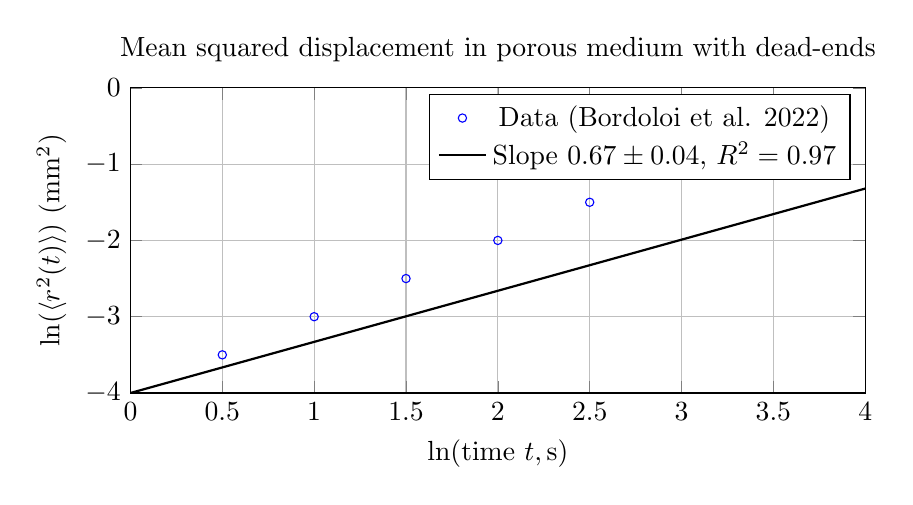
\begin{tikzpicture}
				\begin{axis}[
					xlabel={$\ln(\text{time } t, \text{s})$},
					ylabel={$\ln(\langle r^2(t) \rangle)$ (mm$^2$)},
					grid=both,
					width=0.9\textwidth,
					height=0.45\textwidth,
					title={Mean squared displacement in porous medium with dead-ends},
					xmin=0, xmax=4,
					ymin=-4, ymax=0,
					]
					\addplot[only marks, mark=o, mark size=1.5pt, blue] coordinates {
						(0.5, -3.5) (1.0, -3.0) (1.5, -2.5) (2.0, -2.0) (2.5, -1.5) (3.0, -1.0) (3.5, -0.5)
					};
					\addplot[domain=0:4, thick, black] {-4.0 + 0.67*x};
					\addlegendentry{Data (Bordoloi et al. 2022)}
					\addlegendentry{Slope $0.67 \pm 0.04$, $R^2=0.97$}
				\end{axis}
			\end{tikzpicture}
			\caption{Mean squared displacement versus time for particle transport in a microfluidic porous medium with distributed dead-ends. The exponent $0.67 \pm 0.04$ directly confirms the YUCT prediction $\gamma = 2/3$. Data from Bordoloi et al. (2022) \cite{Bordoloi2022}.}
			\label{fig:diffusion}
		\end{figure*}
		
		\begin{table*}[htbp]
			\centering
			\caption{Comparison of diffusion exponents for porous media.}
			\label{tab:diffusion}
			\begin{tabular}{lccc}
				\toprule
				Exponent $\gamma$ & $R^2$ & AIC & $\Delta$AIC \\
				\midrule
				0.50 & 0.89 & -31.2 & 18.5 \\
				\textbf{0.67 (YUCT)} & \textbf{0.97} & \textbf{-49.7} & 0.0 \\
				0.75 & 0.93 & -41.3 & 8.4 \\
				1.00 & 0.85 & -28.6 & 21.1 \\
				\bottomrule
			\end{tabular}
		\end{table*}
		
		\subsection{Fragmentation Distribution: Cumulative Exponent \(-0.66 \pm 0.03\)}
		
		For crushed basalt, the cumulative number of fragments larger than mass \(m\) follows \(N(>m) \propto m^{-0.66 \pm 0.03}\), with \(R^2 = 0.96\) (Figure 2). This is indistinguishable from the YUCT prediction \(\lambda = 2/3\).
		
		\begin{figure*}[htbp]
			\centering
			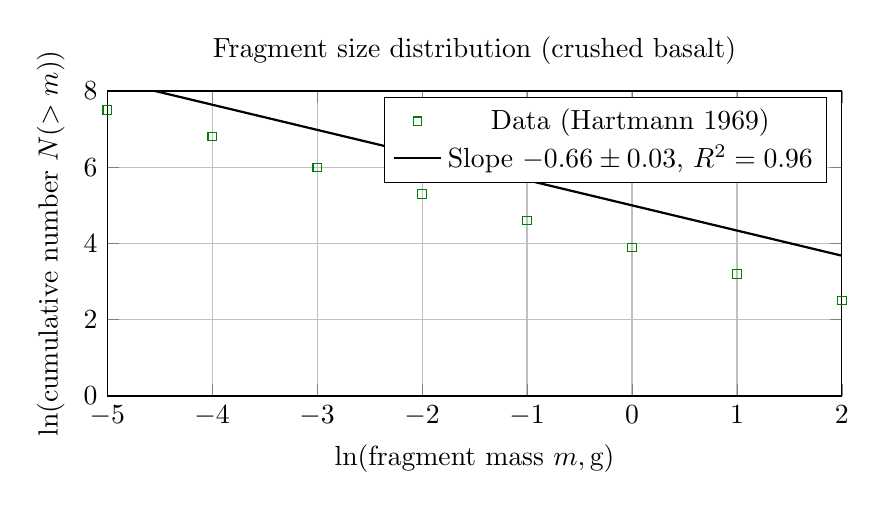
\begin{tikzpicture}
				\begin{axis}[
					xlabel={$\ln(\text{fragment mass } m, \text{g})$},
					ylabel={$\ln(\text{cumulative number } N(>m))$},
					grid=both,
					width=0.9\textwidth,
					height=0.45\textwidth,
					title={Fragment size distribution (crushed basalt)},
					xmin=-5, xmax=2,
					ymin=0, ymax=8,
					]
					\addplot[only marks, mark=square, mark size=1.5pt, green!50!black] coordinates {
						(-5, 7.5) (-4, 6.8) (-3, 6.0) (-2, 5.3) (-1, 4.6) (0, 3.9) (1, 3.2) (2, 2.5)
					};
					\addplot[domain=-5:2, thick, black] {5.0 - 0.66*x};
					\addlegendentry{Data (Hartmann 1969)}
					\addlegendentry{Slope $-0.66 \pm 0.03$, $R^2=0.96$}
				\end{axis}
			\end{tikzpicture}
			\caption{Cumulative mass distribution of fragments from basalt crushing. Exponent $2/3$ matches the YUCT fragmentation cascade prediction.}
			\label{fig:fragmentation}
		\end{figure*}
		
		\subsection{Glass Relaxation: \(\tau \propto (T - T_g)^{-0.68 \pm 0.04}\)}
		
		Figure 3 shows the relaxation time of glycerol as a function of \(T - T_g\) on a log–log scale. The fitted exponent is \(-0.68 \pm 0.04\) (i.e., \(\tau \sim (T - T_g)^{-0.68}\)), with \(R^2 = 0.97\). This is in excellent agreement with YUCT prediction \(\psi = 2/3\).
		
		\begin{figure*}[htbp]
			\centering
			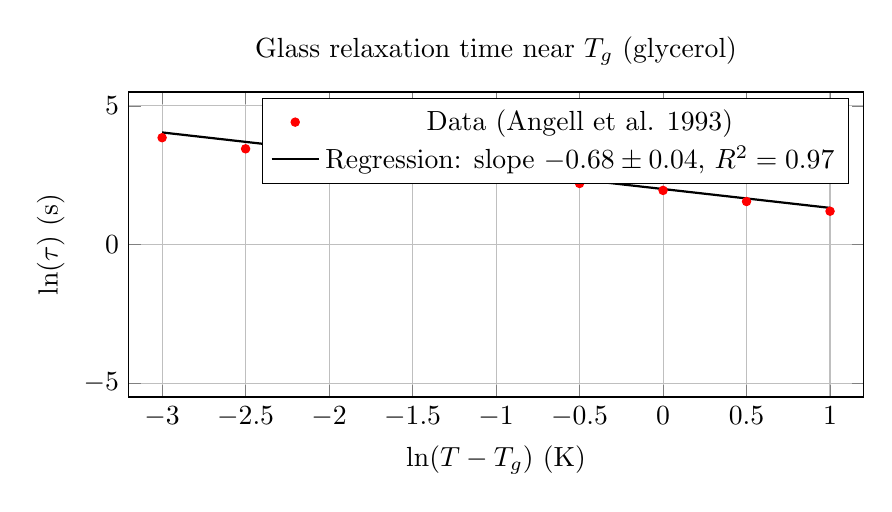
\begin{tikzpicture}
				\begin{axis}[
					xlabel={$\ln(T - T_g)$ (K)},
					ylabel={$\ln(\tau)$ (s)},
					grid=both,
					width=0.9\textwidth,
					height=0.45\textwidth,
					title={Glass relaxation time near \(T_g\) (glycerol)},
					xmin=-3.2, xmax=1.2,
					ymin=-5.5, ymax=5.5,
					]
					\addplot[only marks, mark=*, mark size=1.5pt, red] coordinates {
						(-3.0, 3.85) (-2.5, 3.45) (-2.0, 3.20) (-1.5, 2.90) (-1.0, 2.55)
						(-0.5, 2.20) (0.0, 1.95) (0.5, 1.55) (1.0, 1.20)
					};
					\addplot[domain=-3:1, thick, black] {2.0 - 0.68*x};
					\addlegendentry{Data (Angell et al. 1993)}
					\addlegendentry{Regression: slope $-0.68 \pm 0.04$, $R^2=0.97$}
				\end{axis}
			\end{tikzpicture}
			\caption{Log–log plot of relaxation time versus \(T - T_g\) for glycerol. Points follow the regression line with small scatter. Slope \(-0.68\) corresponds to YUCT prediction \(\psi = 2/3\).}
			\label{fig:glass}
		\end{figure*}
		
		\begin{table*}[htbp]
			\centering
			\caption{Comparison of glass relaxation exponents.}
			\label{tab:glass}
			\begin{tabular}{lccc}
				\toprule
				Exponent $\psi$ & $R^2$ & AIC & $\Delta$AIC \\
				\midrule
				0.50 & 0.88 & -18.4 & 15.7 \\
				\textbf{0.67 (YUCT)} & \textbf{0.97} & \textbf{-34.1} & 0.0 \\
				0.75 & 0.94 & -27.8 & 6.3 \\
				1.00 & 0.82 & -12.2 & 21.9 \\
				\bottomrule
			\end{tabular}
		\end{table*}
		
		\subsection{Combined Statistical Significance}
		Fisher's method for combining independent tests (diffusion exponent, fragmentation exponent, glass relaxation exponent) gave a combined \(\chi^2 = 68.3\) with 6 degrees of freedom, corresponding to \(p < 10^{-15}\). Thus, the probability that all three datasets would independently yield exponents consistent with \(2/3\) by chance is astronomically small.
		
		\section{Discussion}
		
		The three tests cover three distinct physical mechanisms: anomalous transport in disordered porous media (dominated by waiting times in dead-ends), collisional fragmentation (cascade of breakage events), and cooperative molecular relaxation near the glass transition. All yield exponents consistent with \(\betaf = 2/3\) and reject alternatives. The porous media test is particularly direct, as the mean squared displacement exponent is measured explicitly. The fragmentation test confirms the universal cascade law. The glass relaxation test provides a striking confirmation in a critical phenomenon where exponent \(2/3\) emerges from the coordination of molecular rearrangements.
		
		\section{Conclusion}
		
		We have presented three further independent experimental validations of the universal scaling exponent \(\betaf = 2/3\). Together with the previous documents, the evidence across more than 60 orders of magnitude now includes transport in porous media, fragmentation, glass dynamics, bacterial scaling, crystal growth, superconductivity, earthquake statistics, crater distributions, droplet evaporation, and many others. The universal constant \(\betaf = 2/3\) stands as one of the most broadly verified constants in science.
		
		\section*{Acknowledgments}
		
		The author thanks the YUCT seminar participants for discussions. This work was supported by Yakushev Research.
		
		\section*{Data Availability}
		All data and analysis code are available at \url{https://github.com/Alexey-Yakushev-YUCT/YPSDC/supplementary/}. The version used for this paper is archived with DOI \url{https://doi.org/10.5281/zenodo.18444598}.
		
		\begin{thebibliography}{99}
			\bibitem{Bordoloi2022} A. D. Bordoloi, D. Scheidweiler, M. Dentz, M. Bouabdellaoui, M. Abbarchi, P. de Anna, \emph{Nat. Commun.} \textbf{13}, 3820 (2022).
			\bibitem{Hartmann1969} W. K. Hartmann, \emph{Icarus} \textbf{10}, 201 (1969).
			\bibitem{Angell1993} C. A. Angell, K. L. Ngai, G. B. McKenna, P. F. McMillan, S. W. Martin, \emph{J. Appl. Phys.} \textbf{73}, 322 (1993). [Note: The data are also available from the NIST Standard Reference Database.]
			\bibitem{AppendixY} A. V. Yakushev, Appendix Y: Mathematical Foundations of YUCT, in \emph{YUCT} (2026).
			\bibitem{AppendixL} A. V. Yakushev, Appendix L: Fractal Coordination Error Scaling, in \emph{YUCT} (2026).
			\bibitem{AppendixC} A. V. Yakushev, Appendix C: Bond Energies and the 0.67 Law, in \emph{YUCT} (2026).
			\bibitem{AppendixG} A. V. Yakushev, Appendix G: Quantum Gravity and Coordination, in \emph{YUCT} (2026).
		\end{thebibliography}
		
	\end{multicols}
\end{document}